\documentclass[a4paper,12pt]{article}
\usepackage{graphicx}
\usepackage{epstopdf}
\usepackage{gensymb}
\usepackage{float}
\usepackage{listings}

\usepackage[T1]{fontenc}
\usepackage[utf8]{inputenc}


%% Definitioner för LIPS-dokument

\usepackage[swedish]{babel}
\usepackage[utf8]{inputenc}
\usepackage[T1]{fontenc}
\usepackage{times}
\usepackage{ifthen}

\usepackage[margin=25mm]{geometry}

\usepackage{fancyhdr}
\pagestyle{fancy}
\lhead{}
\chead{\textbf{\LIPSprojekttitel}}
\rhead{\textbf{\textsl{LiTH}}\\\textbf{\LIPSdatum}}
\lfoot{\textbf{\LIPSkursnamn}\\\textbf{\LIPSdokumentansvarig}}
\cfoot{\textbf{\LIPSprojektgrupp}\\\textbf{\LIPSgruppepost}}
\rfoot{\textbf{\textsc{Lip}s}\\\textbf{Sida~\thepage}}

\setlength{\parindent}{0pt}
\setlength{\parskip}{1ex plus 0.5ex minus 0.2ex}


\newcommand{\twodigit}[1]{\ifthenelse{#1<10}{0}{}{#1}}
\newcommand{\dagensdatum}{\number\year-\twodigit{\number\month}-\twodigit{\number\day}}

%% ------------------------------------------
% NYBILD
% Skapar centrerad bild med caption
%   
% #1: Filens url relativt '/bilder/'
% #2:  Caption
% #3: Label
% #4: Skalning
%% ------------------------------------------
\newcommand{\nyBild}[4] 
{\begin{figure}[H]
  \centering
 \includegraphics[angle=0,scale=#4]{bilder/#1}
  \caption{#2}
  \label{fig:#3}
\end{figure}}



%%  Redefinitions of commands containing @
\makeatletter
\makeatother

\newcommand{\LIPStitelsida}{%
{\ }\vspace{45mm}
\begin{center}
  \textbf{\Huge \LIPSdokumenttyp}
\end{center}
\begin{center}
  {\Large Redaktör: \LIPSredaktor}
\end{center}
\begin{center}
  {\Large \textbf{Version \LIPSversion}}
\end{center}
\vfill
\begin{center}
  {\large Status}\\[1.5ex]
  \begin{tabular}{|*{3}{p{40mm}|}}
    \hline
    Granskad & \LIPSgranskare & \LIPSgranskatdatum \\
    \hline
    Godkänd & \LIPSgodkannare & \LIPSgodkantdatum \\
    \hline
  \end{tabular}
\end{center}
\newpage
}


\newenvironment{LIPSprojektidentitet}{%
{\ }\vspace{45mm}
\begin{center}
  {\Large PROJEKTIDENTITET}\\[0.5ex]
  {\small
  \LIPSartaltermin, \LIPSprojektgrupp\\
  Linköpings Tekniska Högskola, ISY
  }
\end{center}
\begin{center}
  {\small Gruppdeltagare}\\
%  \begin{tabular}{|p{30mm}|p{40mm}|p{35mm}|p{45mm}|}
  \begin{tabular}{|l|p{45mm}|p{25mm}|l|}
    \hline
    \textbf{Namn} & \textbf{Ansvar} & \textbf{Telefon} & \textbf{E-post} \\
    \hline
}%
{%
    \hline
  \end{tabular}
\end{center}
\begin{center}
  {\small
    \textbf{E-postlista för hela gruppen}: \LIPSgruppepost\\
    \textbf{Hemsida}: \LIPSgrupphemsida\\[1ex]
    \textbf{Kund}: \LIPSkund\\
    \textbf{Kontaktperson hos kund}: \LIPSkundkontakt\\
    \textbf{Kursansvarig}: \LIPSkursansvarig\\
    \textbf{Handledare}: \LIPShandledare\\
  }
\end{center}
\newpage
}
\newcommand{\LIPSgruppmedlem}[4]{\hline {#1} & {#2} & {#3} & {#4} \\}



\newenvironment{LIPSdokumenthistorik}{%
\begin{center}
  Dokumenthistorik\\[1ex]
  \begin{small}
    \begin{tabular}{|l|l|p{60mm}|l|l|}
      \hline
      \textbf{Version} & \textbf{Datum} & \textbf{Utförda förändringar} & \textbf{Utförda av} & \textbf{Granskad} \\
      }%
    {%
      \hline
    \end{tabular}
  \end{small}
\end{center}
}
\newcommand{\LIPSversionsinfo}[5]{\hline {#1} & {#2} & {#3} & {#4} & {#5} \\}

\newcounter{LIPSkravnummer}
\newcounter{LIPSunderkravnummer}[LIPSkravnummer]
\newenvironment{LIPSkravlista}{%
  \begin{tabular}{|p{25mm}|p{25mm}|p{85mm}|p{5mm}|}
    }%
  {%
    \hline
  \end{tabular}
}
\newcommand{\LIPSkrav}[3]{\hline\stepcounter{LIPSkravnummer}\textbf{Krav nr \arabic{LIPSkravnummer}} & \textbf{{#1}} & {#2} & \textbf{{#3}} \\}
\newcommand{\LIPSunderkrav}[3]{\hline\stepcounter{LIPSunderkravnummer}\textbf{Krav nr \arabic{LIPSkravnummer}\Alph{LIPSunderkravnummer}} & \textbf{{#1}} & {#2} & \textbf{{#3}} \\}





%%% Local Variables: 
%%% mode: latex
%%% TeX-master: "kravspec_mall"
%%% End: 



\newcommand{\LIPSartaltermin}{2012/VT}
\newcommand{\LIPSkursnamn}{TSEA27}

\newcommand{\LIPSprojekttitel}{Komborobot}

\newcommand{\LIPSprojektgrupp}{Grupp 17}
\newcommand{\LIPSgruppepost}{komborobot@googlegroups.com}
\newcommand{\LIPSgrupphemsida}{finns ej}
\newcommand{\LIPSdokumentansvarig}{Mattias Jansson}

\newcommand{\LIPSkund}{ISY, Linköpings universitet, 581\,83 Linköping}
\newcommand{\LIPSkundkontakt}{Tomas Svensson, 013-281368, tomass@isy.liu.se}
\newcommand{\LIPSkursansvarig}{Tomas Svensson, 013-281368, tomass@isy.liu.se}
\newcommand{\LIPShandledare}{Olov Andersson, 013-282658, olov@isy.liu.se}


\newcommand{\LIPSdokumenttyp}{Teknisk Dokumentation}
\newcommand{\LIPSredaktor}{Simon Larsson}
\newcommand{\LIPSversion}{1.0}
\newcommand{\LIPSdatum}{\dagensdatum}

\newcommand{\LIPSgranskare}{johjo939}
\newcommand{\LIPSgranskatdatum}{2012-05-10}
\newcommand{\LIPSgodkannare}{}
\newcommand{\LIPSgodkantdatum}{}

\begin{document}

\LIPStitelsida

%% Argument till \LIPSgruppmedlem: namn, roll i gruppen, telefonnummer, epost
\begin{LIPSprojektidentitet}
  \LIPSgruppmedlem{Simon Larsson}{Projektledare (PL)}{070-7311646}{simla804@student.liu.se}
  \LIPSgruppmedlem{\LIPSdokumentansvarig}{Dokumentansvarig (DOK)}{073-6837074}{matja307@student.liu.se}
  \LIPSgruppmedlem{Gustav Svensk}{Reglersystem (REG)}{073-6208776}{gussv666@student.liu.se}
  \LIPSgruppmedlem{Johan Jönsson}{Mjukvara (KA)}{073-8305758}{johjo939@student.liu.se}
  \LIPSgruppmedlem{Tobias Andersson}{Hårdvara (HV)}{073-7201098}{toban963@student.liu.se}
  \LIPSgruppmedlem{Markus Falck}{Leveransansvarig (LV)}{076-3457552}{marlo265@student.liu.se}
  \LIPSgruppmedlem{Simon Wallin}{Testansvarig (GM)}{076-2300665}{simwa252@student.liu.se}
\end{LIPSprojektidentitet}

\tableofcontents{}
\newpage

%% Argument till \LIPSversionsinfo: versionsnummer, datum, ändringar, utfört av, granskat av
\addcontentsline{toc}{section}{Dokumenthistorik}
\begin{LIPSdokumenthistorik} 
  \LIPSversionsinfo{0.1}{2012-04-10}{Första utkast.}{gussv666}{}
  \LIPSversionsinfo{0.2}{2012-05-06}{Nya rubriker.}{matja307}{}
  \LIPSversionsinfo{1.0}{2012-05-10}{Slutgiltig version}{matja307}{johjo939}
\end{LIPSdokumenthistorik}
\newpage 

\section{Inledning}
Text här
 % #1 -Bakgrund och syfte
% !TEX encoding = UTF-8 Unicode

%% --------------------------------------------------------------------------------------------------------------------------------------------
% PRODUKTEN - En översiktlig beskrivning av produkten och hur den fungerar, samt vad den används till.
%
% - Inledande beskrivning av funktionalitet
% - Bild på produkten
% - Översikt över systemet
%
% --matja307, 2012-05-06
%% --------------------------------------------------------------------------------------------------------------------------------------------
 
\section{Översikt av produkten}

Roboten är en s.k. \emph{komborobot}, vilket innebär att den dels kan följa en 
linje på marken, dels ta sig igenom en labyrint. Roboten kan vidare autonomt 
växla mellan linje- och labyrintläge, samt uppfatta en speciell stoppsignal som
markeras med linjer på marken. Roboten kan också styras manuellt via bluetooth 
från en PC, samt skicka relevant information, såsom sensordata, till PC. 

Figur \ref{fig:prod1} visar robotens utseende. Basen är en trehjulig plattform 
av typ \emph{CarpetRover}, på vilken är monterat fem stycken avståndssensorer 
riktade åt sidorna respektive framåt, samt x stycken sensorer för att upptäcka 
linjer på marken. 

\nyBild{produktbild.png}{Bild på produkten}{prod1}

Robotens funktionalitet är uppdelad på tre enheter, som var och en 
representeras av en AVR-processor. De tre enheterna är: 
\begin{itemize}
        \item Kommunikationsenhet
        \item Sensorenhet
        \item Styrenhet
\end{itemize}

All intern kommunikation sker via en SPI-buss. 
Kommunikationsenheten fungerar som master på bussen, det vill säga att all 
kommunikation går via den. Bluetooth-kommunikationen med PC sköts också i 
kommunikationsenheten.
 % #2 -Översikt
% !TEX encoding = UTF-8 Unicode

%% --------------------------------------------------------------------------------------------------------------------------------------------
% Protokoll - En beskrivning av de protokoll som används för kommunikationen, och vad de är bra för.
%
%
% --marlo265, 2012-05-06
%% --------------------------------------------------------------------------------------------------------------------------------------------
 
\section{Protokoll}
\label{sec:protokoll}

För att förenkla kommunikation mellan enheter så används ett enhetligt
protokoll, detta gör det också väldigt mycket lättare att lägga till fler
enheter till roboten.


\subsection{Generell överföring mellan enheter}
Kommunikationen mellan de olika enheterna sker via en SPI-buss (se 
\ref{sec:SPI}).
All kommunikation består av en headerbyte följt av en databyte.
I headerbyten anges till vilken enhet den efterföljande informationen ska, 
samt hur den ska tolkas av den mottagande enheten.
De tre mest signifikanta bitarna i headern anger till vilken enhet 
informationen ska och de 5 minst signifikanta bitarna anger 
hur denna information ska behandlas. Uppdelningen kan ses i tabell 
\ref{tab:header}.  Kodningen av de tre mest signifikanta bitarna kan ses i 
tabell \ref{tab:headerkod}.

All kommunikation går via kommunikationsenheten, så om sensorenheten vill 
skicka data till styrenheten skickar den en headerbyte med styrenhetens adress 
och en databyte till kommunikationsenheten som 
tolkar headern och skickar headern och databyten till styrenheten.
\begin{table}[h]
  \centering
  \begin{tabular}{| c | c | c | c | c | c |}
    \hline
    Målenhet [3 bitar] & A & B & C & D & E \\
    \hline
  \end{tabular}
  \caption{Bituppdelning av header}
  \label{tab:header}
\end{table}

\begin{table}[h]
  \centering
  \begin{tabular}{l l}
    \textbf{3 MSB} & \textbf{Målenhet} \\
    000 & Kommunikationsenhet \\
    001 & Sensorenhet \\
    010 & Styrenhet \\
    100 & PC \\
    110 & PC och Styrenhet\\
  \end{tabular}
  \caption{Kodning av header}
  \label{tab:headerkod}
\end{table}


\subsection{PC-mjukvara $\longleftrightarrow$ Styrenhet}
Då styr- eller sensorenheten sänder data till PC-mjukvaran kommer mjukvaran att
översätta header-byten samt data-byten så att man enkelt kan åskådliggöra
instruktionen som sändes. 
PC-mjukvaran skickar styrkommandon till roboten då roboten är i fjärrstyrt läge.
Bituppdelningen av styrkommandon kan ses i tabell \ref{tab:styrbitar} och
kodningen kan ses i tabell \ref{tab:styrkommando}.

Om styrenheten får en header den inte känner igen så skickar den ett
felmeddelande till PCn.

\begin{table}[h] 
  \centering
  \begin{tabular}{| c | c |}
    \hline
    Kommando [4 bitar] & Hastighet [4 bitar] \\ \hline
  \end{tabular}
  \caption{Bituppdelning av styrkommandon}
  \label{tab:styrbitar}
\end{table}

\begin{table}[h] 
  \centering
  \begin{tabular}{l l}
    \textbf{4 MSB} & \textbf{Kommando} \\
    0000 & Stopp \\
    0001 & Framåt \\
    0010 & Fram vänster \\
    0011 & Fram höger \\
    0100 & Rotera vänster \\
    0101 & Rotera höger \\
    0110 & Back \\
    0111 & Set_left \\
    1000 & Set_right \\
    1001 & Trim_left \\
    1010 & Trim_right \\
    1011 & No_trim \\
  \end{tabular}
  \caption{Kommandokodning}
  \label{tab:styrkommando}
\end{table}


\subsection{PC-mjukvara $\longleftrightarrow$ Sensorenhet}
När sensorenheten skickar information till styrenheten och PCn 
så anger E-flaggan om roboten är i autonomt eller fjärrstyrt läge.
D-flaggan avgör om databyten som mottagits är ett specialkommando eller inte.
A-flaggan anger om roboten kör i labyrint eller om den följer en linje.
Flaggornas lägen kan ses i tabell \ref{tab:adeflaggor}.


PC-mjukvaran skickar data till sensorenheten då tröskelvärdet på linjesensorerna
kalibreras, se \ref{sec:linjesensor}.

\begin{table}[h]
  \centering
  \begin{tabular}{l l l l l l l l}
    \textbf{A} & \textbf{Läge} & & \textbf{D} & \textbf{Typ av data} & & \textbf{E} & \textbf{Läge} \\
    0 & Labyrint & & 0 & Sensordata & & 0 & Fjärrstyrt \\
    1 & Linje & & 1 & Specialkommando & & 1 & Autonomt \\
  \end{tabular}
  \caption{A-,D- och E-flaggor}
  \label{tab:adeflaggor}
\end{table}


\subsection{Sensorenhet $\longleftrightarrow$ Kommunikationsenhet}
Sensorenheten skickar data till kommunikationsenheten som ska vidare både 
till PCn och styrenheten. Detta anges med en header enligt tabell 
\ref{tab:headerkod}. Efterföljande data är antingen ett specialkommando, se 
tabell \ref{tab:special}, avstånd till väggar eller avstånd till centrumlinjen.

\begin{table}[h] 
  \centering
  \begin{tabular}{| c | c | c | c | c | c |}
    \hline
     0 & Specialkommando [3 bitar] & 0 & 0 & 0 & 0 \\ \hline
  \end{tabular}
  \caption{Bituppdelning av specialkommandon}
  \label{tab:specialbitar}
\end{table}

\begin{table}[h]
  \centering
  \begin{tabular}{l l}
    \textbf{Kodning} & \textbf{Specialkommando} \\
    000 & Återuppta vanlig reglering\\
    001 & Kör rakt fram \\
    010 & Sväng höger 90\degree \\
    011 & Sväng vänster 90\degree \\
    100 & Rotera höger 90\degree \\
    110 & Rotera vänster 90\degree \\
  \end{tabular}
  \caption{Kodning av specialkommandon}
  \label{tab:special}
\end{table}

 % #3 - Protokoll
%% --------------------------------------------------------------------------------------------------------------------------------------------
% SYSTEMET - �versiktligt blockschema f�r systemet i sin helhet, samt �vergripande information om densamma.
%
% --matja307, 2012-05-06
%% --------------------------------------------------------------------------------------------------------------------------------------------

\section{Systemet}

De tre huvudenheterna styrs av varsin AVR-processor (ATmega16), vilka klockas 
av en gemensam extern EXO-3 kristalloscillator. Sensorenheten läser av och 
tolkar värden från sensorerna och skickar denna information till 
kommunikationsenheten, som i sin tur skickar datan vidare till styrenheten 
och PC-mjukvaran. Styrenheten tolkar sensordatan från 
sensorenheten (i autonomt läge) eller styrkommandon från PC-mjukvaran 
(i fjärrstyrt läge) och styr de två motorerna som driver var sitt av de två 
främre hjulen på pattformen. Information från avståndssensorerna skickas även
till PC-mjukvaran och den inbyggda displayen, på vilka avståndet till 
närliggande väggar visas i centimeter.  Ett skjutreglage på robotens ovansida 
avgör om roboten navigerar själv med hjälp av sensordata (autonomt läge), 
eller om den styrs via fireflyenheten med den medföljande PC-programvaran. 
Dessutom finns på ovansidan en knapp för att starta roboten då den är i autonomt läge 
(svart knapp) samt en resetknapp (röd knapp).

\begin{figure}[H]
 \centering
 %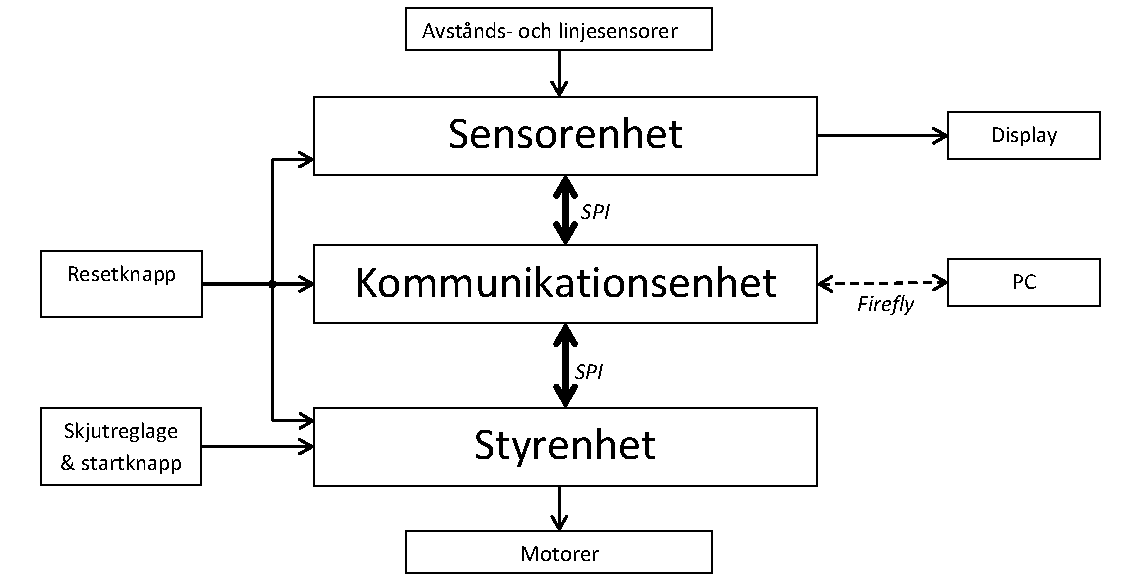
\includegraphics[angle=0,scale=0.8]{bilder/systemoversikt.pdf}
  \caption{Översikt av systemet}
  \label{fig:system}
\end{figure}


\subsection{Kommunikation}
All intern kommunikation sker via en SPI-buss. Kommunikationsenheten fungerar 
som master på bussen, och all kommunikation går via den. När en enhet vill 
kommunicera med en annan kommer aviseras detta genom att enheten genererar 
ett avbrott på kommunikationsenheten.  Robotens kommunikation med PC-
mjukvaran sker via bluetooth.
 % #5 -Blockschema och allmänt om systemet i sin helhet
%% --------------------------------------------------------------------------------------------------------------------------------------------
% MODULERNA - Bara inkludering av dokument f�r modulerna.
%
% --matja307, 2012-05-06
%% --------------------------------------------------------------------------------------------------------------------------------------------

% !TEX encoding = UTF-8 Unicode
%% --------------------------------------------------------------------------------------------------------------------------------------------
% KOMMUNIKATIONSENHETEN - Detaljbeskrivning av kommunikationsenheten
%
% --matja307, 2012-05-06
%% --------------------------------------------------------------------------------------------------------------------------------------------

\section{Kommunikationsenhet}

Kommunikationsenheten ansvarar för att förmedla data mellan de olika 
enheterna i systemet. Kommunikationsenheten består av en AVR ATmega16 och en 
Fireflymodul. Processorn klockas av en extern 16 MHz, samma klocka som för 
resten av systemet. Kommunikationsenheten tar ingen hänsyn till om roboten 
opererar i fjärrstyrt eller autonomt läge.

Kommunikationen mellan PCn och roboten sker via blåtand. Kommunikation mellan 
de olika enheterna på roboten sker med en så kallad SPI-buss. SPI-bussens 
olika anslutningar kan betraktas i figur \ref{fig:spibuss}. Hur de olika 
pinnarna på processorn är anslutna kan betraktas i figur \ref{fig:PINkomm}.

\begin{figure}[H]
  \centering
 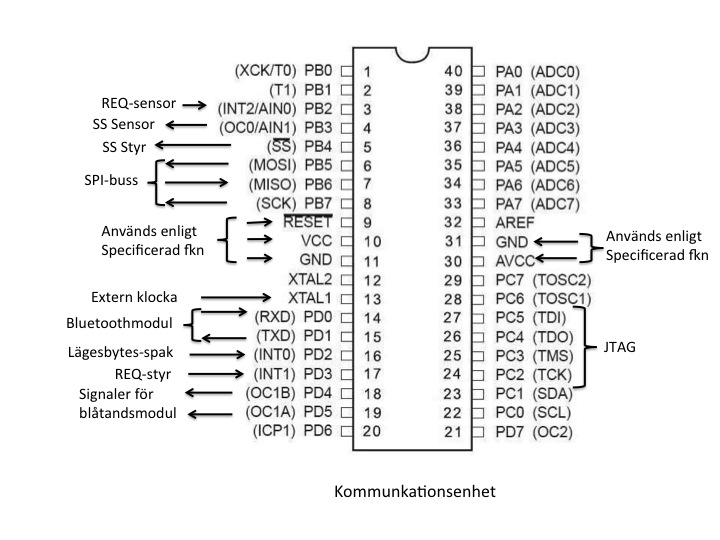
\includegraphics[angle=0,scale=0.5]{bilder/PIN_komm.jpg}
  \caption{Kommunikationsenhetens pin-anslutningar}
  \label{fig:PINkomm}
\end{figure}

\subsection{Bluetooth}
%Övevrsikt
Roboten kommunicerar med PCn med Bluetooth via enheten \emph{FireFly Bluetooth Modem - BlueSMiRF Gold}. Överföringen mellan kommunikationsenhetens AVR-processor och Firefly-enheten sker seriellt med protokollet RS232 via mikroprocessorns USART-register. 

%Överföring från AVR
Bluetooth-överföringen till och från Firefly-enheten använder fyra pinnar på mikroprocessorn: RTS, CTS, RXD samt TXD, se fig. \ref{fig:PINkomm}. Data skickas och tas emot på TXD respektive RXD. RTS- och CTS-signalerna används för att signalera när data ska skickas och tas emot. Överföringen sker i asynkront läge med en baude rate på 115200 bps. Förutom de åtta databitarna så skickas även en start- och en stoppbit. Inga paritetsbitar används. 

%Ta emot data
\subsubsection*{Ta emot data}
Då ingen data skickas eller tas emot så väntar enheten på att ta emot data. Efter det att en byte mottagits så sker ett avbrott av typen \emph{Recieve complete interrupt}. Som beskrivs i sektion \ref{sec:SPI} så sker all kommunikation med två bytes. På grund av detta så väntar kommunikationsenheten i avbrottet på att ta emot ytterligare ett ord. När detta tagits emot så vidarebefordras de två orden till bussen. 

%Skicka data
\subsubsection*{Skicka data}
Vid varje överföring skickas två bytes, ett header- och ett dataord. Detta kräver alltså två separata överföringar om åtta bitar. Då det första ordet skrivits till \emph{UDR-registret} så väntar processorn på att flaggan \emph{TXC, Transmit complete} sätts, varpå nästa ord skrivs till registret. Då båda orden överförts så sätts åter enheten att lyssna på mottagen data. 

\subsection{SPI}
\label{sec:SPI}
SPI bussen är ett kommunikationssystem som använder ett så kallat 
Master-Slav system. I robotens SPI-buss är kommunikationsenheten ensam Master.
SPI-bussen har två slavar i form av styrenheten och sensorenheten. För att 
ställa in huruvida en enhet ska agera master eller slav modifieras på Atmega16 
innehållet i kontrollregistrer för SPI-bussen, SPCR. SPI-bussen arbetar alltid 
i så kallat full duplex läge vilket betyder att överföringar kan ske i två 
riktningar samtidigt. Alla överföringar i systemet sker med två bytes åt 
gången, en headerbyte som bland annat innehåller adressen och en databyte. 
När kommunikationsenheten avslutat en överföring så analyseras alltid 
headerbyten, som mottagits genom tvåvägskommunikationen, innan nästa 
överföring behandlas.  


Robotens kommunikationssystem fungerar så att styr- och sensorenheten har 
möjlighet att ta initiativ till överföringar till och från 
kommunikationsenheten. Detta är inte standard på SPI-bussen utan löses med två 
stycken extrasignaler, så kallade Request-signaler. Alla sorters kommunikation 
kommer att styras med hjälp av avbrott, vilket är ett utmärkt sätt att hantera 
plötsliga externa kommandon. Då någon av slavarna vill påbörja en överföring 
sätts enhetens REQ signal hög, vilket genererar ett avbrott hos mastern. Är 
mastern upptagen då en hög REQ signal skickas så får enheten vänta på att 
mastern avslutat den pågående överföringen. Efter att mastern blivit 
uppmärksammad om att en överföring efterfrågas sätts SS-signalen till den 
berörda enheten låg. Överföringen startas i det ögonblick som mastern skriver 
något till det temporära SPI-registret, SPDR. I detta ögonblick så börjar 
mastern också dela ut en klockpuls för överföringen till slavarna. I detta 
läge och framåt görs ingen skillnad på huruvida det var slaven eller mastern 
som initierade överföringen. Alla SPI-överföringar avslutas med att en speciell
avbrottsflagga, kallad SPIF, sätts. När detta sker kommer båda parterna i 
överföringen att spara undan den mottagna datan. Då alla SPI överföringar sker 
med 8 bitar upprepas denna procedur två gånger för varje överföring.

Nedan följer klargöranden om hur de olika portarna i SPI-bussen används, samt 
vilka register som används och hur dessa programmeras. 

\subsubsection{SPI-bussens portar}

Atmel Atmega16 har hårdvarustöd för SPI-bussar. Detta betyder i praktiken att 
det finns pinnar på processorn som enkelt kan ställas in för att fungera 
enligt SPI-standard. Dessa pinnar ligger alla på Port B, se \ref{fig:PINkomm}.
I \ref{fig:spibuss} visas hur pinnarna i de olika enheterna ska kopplas samman.

\begin{figure}[H]
  \centering
 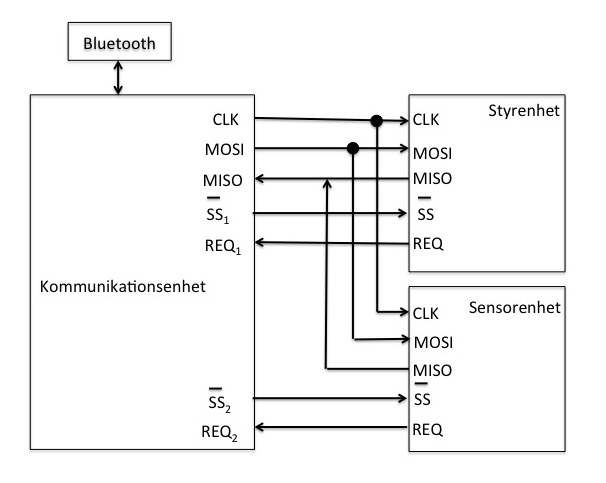
\includegraphics[angle=0,scale=0.5]{bilder/SPI-buss.png}
  \caption{SPI-bussens olika anslutningar. }
  \label{fig:spibuss}
\end{figure}


\textbf{SCK}


SCK porten är en port som förmedlar en klocka med en viss frekvens från 
mastern till de två slavarna. Denna signal bestämmer hur snabbt överföringen 
ska ske. Klockan kommer börjar skickas då mastern skriver något till dess 
temporära SPI dataregister, SPDR. När detta skett skickas totalt 8 pulser 
vilket överför 8 bitar i båda riktningar. Mastern och slavarna måste 
konfigureras för att överföringens olika skeden ska ske samtidigt i 
klockcykeln. Robotens enhet är konfigurerade för att börja med överföring av 
MSB i det temporära SPI-registret SPDR. SCK signalen är konfigurerad till att 
vara låg då ingen överföring sker.

I robotens SPI-buss används frekvensen 4 MHz, det vill säga 1/4-del av 
enheternas arbetsklockan på 16 MHz, för överföringar. Detta är den snabbast 
möjliga överföringshastigheten som garanteras av tillverkaren Atmel. Vid 
behov finns också möjlighet att öka överföringshastigheten till halva 
arbetsklockan, det vill säga 8 MHz. Märk dock att denna överföringshastighet 
inte är garanterad att fungera för slavar.


\textbf{MOSI}


MOSI porten är den port som används när kommunikationsenheten ska skicka 
information till styrenheten och sensorenheten. Den kommer alltså att 
användas som input för slavarna och output för mastern. MOSI-signalen 
parallellkopplas till slavarna, se \ref(fig:spibuss). Om SPI-bussen är 
korrekt inställd kommer slaven som inte är avsedd att motta den skickade 
datan att ignorera vad överföringen. Se pin SS för mer information om 
denna funktion.

\textbf{MISO}


MISO porten används då kommunikationsenheten hämtar information från styr- 
och sensorenheten. Den är alltså att vara en input för mastern och output för 
båda slavarna. Precis som MOSI-signalen porten är MISO-signalerna 
parallellkopplade till slavarna.  Då all kommunikation med SPI är tvåsidig 
används även MOSI porten varje gång MISO porten används och viceversa. En 
slav som inte är vald genom en hög SS-signal, se nedan, kommer inte 
att kunna skicka något via MISO-porten. 

\textbf{SS}
\label{sec:SS}


SS portarna skickar eller tar emot en variant på en chip-select signal. Den SS
-signal som är låg väljer vilken av slavarna som mastern ska kommunicera med. 
Endast en av de två SS signalerna får vara låg samtidigt, detta för att 
undvika busskonflikter. Dessa portar kommer att vara output på mastern(
kommuikationsenheten) och input på styr- och sensorenheten(slavarna).

En låg SS signal hos någon av slavarna betyder att slavens SPI är aktiverad, 
förutsatt att nödvändiga bitar satts i slavens SPI-kontrollregister 
SPCR. Överföringen kommer inte att startas förens mastern skriver data till 
dess temporära dataregister SPDR. Överöringens start genererar inget avbrott 
hos slaven, utan sker istället parallellt med övrig aktivitet hos slaven. Då 
överföringen avslutats genereras ett avbrott där slaven sparar undan den 
skickade byten. Detta avbrott initieras genom att flaggan SPIF sätts hög. En 
enhet som får en hög SS signal kommer att ha sin SPI inaktiv och kommer inte 
att påverkas av aktivitet på databussen. Efter att två bytes överförts sätts 
SS signalen åter hög och mastern påbörjar en analys av den skickade headern 
och om denna specificerar att den mottagna datan ska skickas någonstans.

\textbf{REQ}


REQ portarna används av styr- och sensorenheten för att uppmärksamma 
kommunikationsenheten om att de har ny data att förmedla. När 
kommunikationsenheten tar emot en hög signal på någon av REQ portarna kommer 
det att generera ett avbrott. Detta möjliggörs genom att REQ-signalerna är 
inkopplade till portar på kommunikationsenheten som kan programmeras till att 
generera avbrott vid förändringar. Under avbrottet kommer SS signalen till 
enheten som begärt kommunikation att sättas låg och kommunikationen påbörjas. 
Då mastern kan vara upptagen i det ögonblick då den mottar en hög REQ-signal 
så låter slavarna REQ-signalen vara hög tills dess att överföringen är färdig 
då den sätts låg.

REQ-signalen används också för att bekräfta att slavarna sparat undan en 
headerbyte och är redo att ta emot en databyte. 

\subsubsection{SPI-register på Atmega16}

Det finns i Atmega16 flertalet register som används för att kontrollera SPI-
bussen. Dessa register varierar lite i funktion beroende på om processorn är 
inställd för att fungera som master eller slav på SPI-bussen. För mer 
information om dessa register se *INSERT KÄLLA atmega16 guide*

\textbf{SPI Statusregister - SPSR}


Detta register innehåller dels två olika flaggor och dels en bit som kan 
sättas hög för att fördubbla SPI-bussens överföringshastighet om processorn 
är konfigurerad till att fungera som master . 

MSB är SPIF-flaggan som sätts hög på både master och slav när en 
SPI- överföring slutförts. Tillåts SPI-avbrott kommer 
det att leda till ett avbrott i processorn när denna flagga sätts hög. 
Flaggan rensas genom att denna avbrottsvektor utförs, alternativt genom att 
SPSR läses och därefter läsa från(eller skriva till) SPI-bussens data-register SPDR.

Resten av registrets innehåll används inte i projektet.

\textbf{SPI kontrollregister - SPCR}


Innehållet i detta register avgör om och hur SPI-bussen ska fungera på 
processorn. Endast de bitar som konfigureras i roboten kommer att beskrivas. 
Värt att notera är att robotens överföringshastighet, 1/4 av arbetsklockan, 
uppnås genom att de två minst signifikanta bitarna lämnas låga.

Bit 7 sätts hög för att tillåta avbrott då SPIF sätts hög. Denna bit är satt 
på alla enheter på roboten.

Bit 6 sätts hög för att använda SPI-buss. Sätts inte denna bit hög kommer 
inte SPI-överföringar att fungera.

Bit 4 sätts hög för att göra enheten till master. Det betyder att denna bit 
ska vara hög på kommunikationsenheten men låg på styr- och sensorenheten.

\textbf{SPI dataregister- SPDR}


Detta är ett temporärt 8-bits dataregister som skiftas vid en SPI-överföring. 
Slavar kan skriva till SPDR vid godtyckligt tillfälle. Då mastern skriver 
till SPDR påbörjas överföringen. Då varje överföring i roboten består av två 
skiftningar av SPDR är det viktigt att informationen i SPDR sparas mellan de 
två skiftningarna.


\subsubsection{Exempel}

För att tydliggöra hur bussen fungerar beskrivs nedan ett exempel på hur en 
överföring kan gå till.

När roboten befinner sig i labyrint-läge har sensorenheten gjort en ny 
avläsning som resulterar i beslutet att en 90\degree kurva är nödvändig. Den 
vill distribuera denna information vidare till både styrenheten och PCn som 
övervakar robotens aktivitet. Sensorenheten sätter då en hög utsignal på sin 
REQ port vilket resulterar i ett avbrott på kommunikationsenheten. 
Kommunikationsenheten är för närvarande är för närvarande upptagen med 
överföring av reglerdata till styrenheten, så avbrottet får vänta tills det 
att denna överföring är klar. Under denna väntan är sensorenhetens REQ signal 
fortsatt hög.

I avbrottet på kommunikationsenheten så sätts SS signalen till sensorenheten 
låg, och därefter förmedlar kommunikationsenheten en klockpuls till 
sensorenheten. När två bytes överförts, en headerbyte och en databyte, så 
avslutas överföringen och SS signalen till sensorenheten sätts åter hög. 
Efter att headerbyten tolkats så sätter kommunikationsenheten SS signalen 
till styrenheten låg, samt genererar en klockpuls till styrenheten. När 
överföringen av två bytes är färdig sätts SS signalen till styrenheten 
återigen hög vilket avslutar överföringen via SPI-bussen. 

Då headerbyten innehöll information om att detta var ett styrbeslut så ska 
kommunikationsenheten också skicka detta till PCn. Detta görs via en UART 
port på kommunikationsenheten efter det att headern som skickats från 
styrenheten analyserats. Det är mycket viktigt att en enhet som inte har 
något att skicka vidare sätter innehållet 

De olika enheternas roll i detta exempel åskådliggörs nedan i ett schema, se 
figur \ref{fig:schema}.


\begin{figure}[H]
 \centering
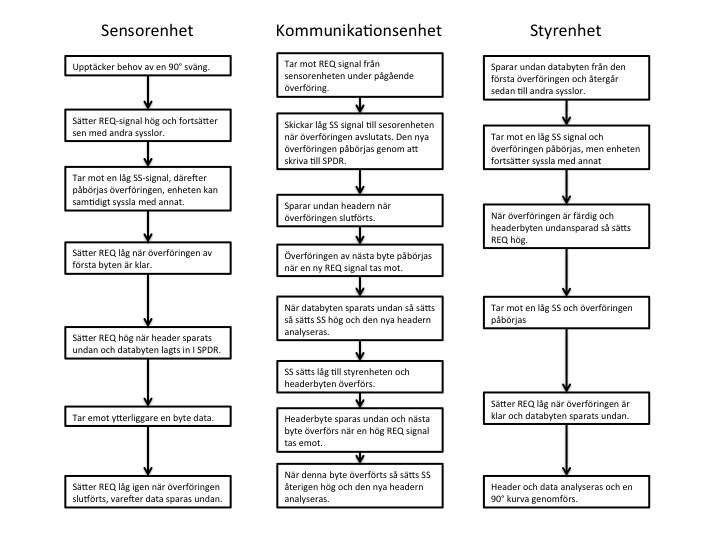
\includegraphics[angle=0,scale=0.7]{bilder/schema_exempel.jpg}
  \caption{Schema över de olika enheternas metodik vid exempelöverföringen}
  \label{fig:schema}
\end{figure}




\section{PC mjukvara}
PC-mjukvaran har som uppgift att låta användaren kommunicera med roboten via ett
enkelt gränssnitt. Via PC-mjukvaran kan användaren få intressant information
från robotens olika moduler, t.ex avstånd till väggar eller vilket styrkommando
som nu utförs. PC-mjukvaran kommunicerar med roboten via blåtand.

\subsection{Implementering}

Mjukvaran är skriven i programspråket C och använder utöver Cs standardbibliotek
även gränssnittet BlueZ för att kommunicera via blåtand, biblioteket SDL för att
generera kommandon till roboten via tangentbordet samt NCurses för att
åskådliggöra information i terminalen på ett trevligt och överskådligt sätt..

Mjukvaran består av 2 huvuddelar, input\_control samt send\_receive. input\_control
hanterar knapptryckningar från användaren och genererar instruktioner att skicka
till roboten, intruktionen placeras sedan i en enkel databas (instr\_db).
send\_receive i sin tur läser in instruktionen från databasen och om användaren
har genererat en ny instruktion kommer denna skickas till roboten via blåtand
(instruktioner som redan skcikat till roboten kommer alltså inte att skickas
 igen), ifall instruktionen innehåller information om önskad hastighet på
roboten eller trimnivåer på motorerna så kommer detta också visas på skärmen.
När instruktionen skickats till roboten kommer send_receive invänta 2 databyte
från roboten (vilket kan vara sensorinfo, specialkommando el. dyl.) som sedan
kommer åskådligjöras på skärmen.
\subsection{Användande}

För att börja använda roboten startar man först programmet input_control, detta
initierar databasen instr\_db och ger användaren möjlighet att skapa
styrkommandon åt roboten med hjälp av tangentbordstryckningar. Sedan startar man
programmet send_receive som ansluter till roboten via blåtand och börjar skicka
samt ta emot data från roboten.

Då roboten befinner sig i fjärrstyrt läge används följande tangentbindningar för
att generera styrkommandon:
w - Kör framåt
s - Kör bakåt
a - rotera vänster
d - rotera höger
q - vänstersväng (mjuk kurva)
e - högersväng (mjuk kurva)
mellanslag - stanna roboten
pil upp - öka hastigheten, ingen effekt tills man skickar ett kommando som
utnyttjar hastigheten
pil ner - sänk hastigheten, ingen effekt tills man skickar ett kommando som
utnyttjar hastigheten.
pil höger - trim höger, öka effekten på höger motor en aning (små steg,
		användbart för finjustering)
pil vänster - trim vänster, öka effekten på vänster motor en aning (små steg,
		användbart för finjustering)
o - nollställ trim
esc - avsluta input\_control

För att avsluta send\_receive används (ctr + c) vilket kommer återställa
terminalen åt användaren.

% \subsection{Implementering}
% 
% Mjukvaran är skriven i programspråken C samt Tcl och använder utöver Cs standardbibliotek
% även gränssnittet BlueZ för att kommunicera via blåtand.
% 
% \subsection{Användande}
% 
% Mjukvaran kommer utgöras av ett fönster där användaren kan se information
% skickad från robotens sensorer och dess styrenhet samt skicka styrkommandon till
% roboten.
% 
% I fjärrstyrt läge kan användaren välja att använda de pilknappar som finns i
% fönstret för att styra roboten eller så kan användaren använda piltangenterna på
% tangentbordet.
% 
% I autonomt läge kommer gränssnittet visa information från robotens sensorer samt
% vilket styrkommando som roboten just nu utför.
% 
% Gränssnittet är enkelt att använda, kommandona är logiska och simpla och
% informationen från roboten visas på ett tydligt och lättförståeligt sätt.
% 

% !TEX encoding = UTF-8 Unicode

\section{Sensorenhet}

Sensorenheten är den enhet som behandlar all sensordata. Den samlar in data från 
avståndssensorerna och linjesensorerna som den sedan antingen omvandlar till 
cm värden i avståndsensorns fall, eller trösklar och ger diskreta varierande storheter 
som i linjesensorns fall. Linje sensorn kommunicerar sedan med kommunikationsenheten
som förmedlar värdena till styrenheten och till PCn.

\subsection{Hårdvara}

\begin{figure}[H]
  \centering
 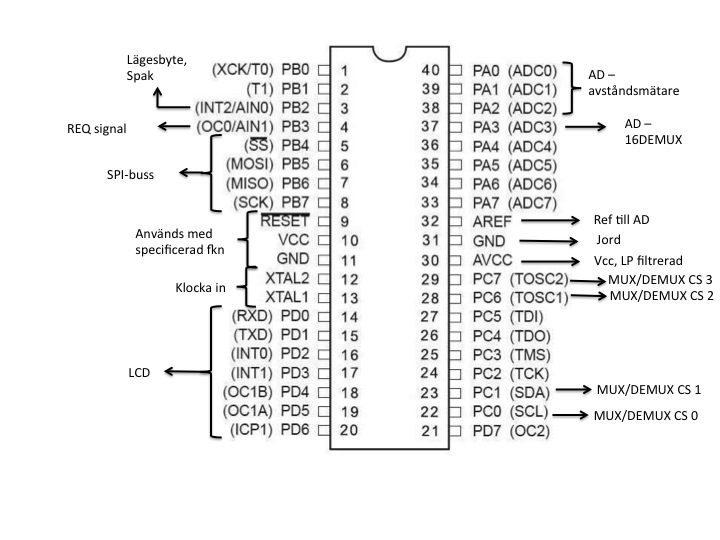
\includegraphics[angle=0,scale=0.5]{bilder/PIN_sensor.jpg}
  \caption{Sensorsenhetens pin-anslutningar}
  \label{fig:PINsensor}
\end{figure}

\subsubsection{Linjeföljarsensor}
För att maximera robotens framförhållning är sensorerna monterade framför roboten 
så långt fram som möjligt ca 3 mm ovanför marken. Linjesensorn består av 11st lysdioder 
med 11st ljuskänsliga transistorer, en multiplex och en demultiplex.

\begin{figure}[H]
  \centering
 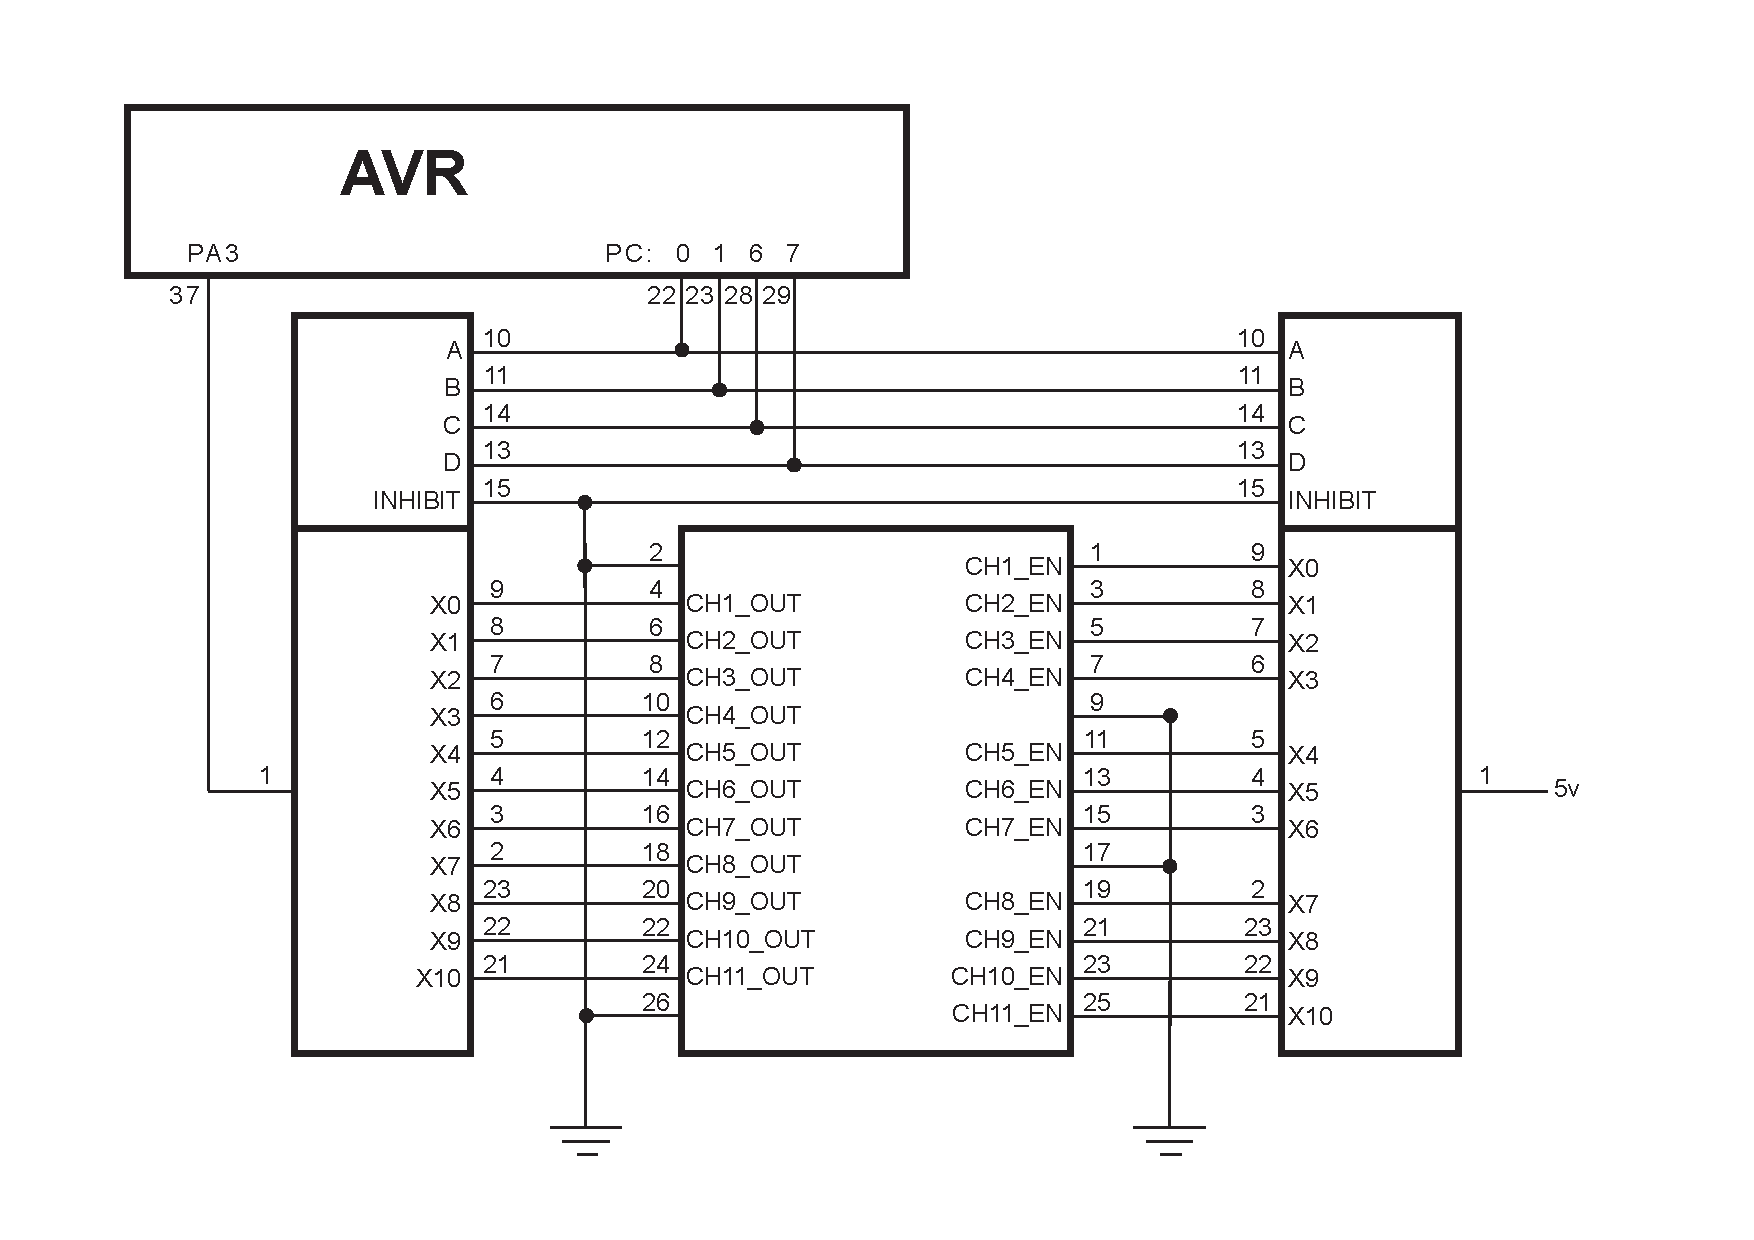
\includegraphics[angle=0,scale=0.5]{bilder/Uppkoppling_linjesensorer.pdf}
  \caption{Uppkoppling linjesensorer}
  \label{fig:Uppkoppling_linjesensorer}
\end{figure}

CH1 EN - CH11 EN är ingångar som leder signalen (logiskt ) vidare till lysdioderna. 
CH1  OUT - CH11 OUT Leder svarssignalen från transistorerna vidare mot styrenhetens 
AVR. Multiplexen och demultiplexen styrs med signalerna A - D från AVRen. Inhibit 
signalen är jordad då dataväljning alltid ska vara tillåten.



\subsubsection{Upptäckning av riktningsmarkeringar}
\label{sec:riktmark}
Då roboten är i en labyrint kommer linjeföljarsensorn huvudsakligen användas 
för att hitta riktningsmarkeringar. Dessa markeringar används för att visa i 
vilken riktning roboten ska färdas i nästkommande korsning.  I enlighet med 
banspecifikationen, se *REF BANSPEC*, är funktionen anpassad för att uppfatta 
följande signaler:

Högersväng visas med en tunn tejpmarkering följd av en tre gånger så tjock.
Vänstersväng visas genom en tjock tejpmarkering följd av en tre gånger så tunn.
Framåt visas genom två tunna tejpmarkeringar.

Vid varje uppdatering av samtliga linjeföljarsensorer görs en kontroll om de 
tre mittersta sensorerna ligger över tejp. Är så fallet så börjar antalet 
gånger linjesensorerna uppdateras att räknas. När de tre mittersta sensorerna 
inte längre ligger över tejp sparas antalet iterationer som sensorerna 
tillbringat över tejpen. Proceduren upprepas därefter och antalet iterationer 
jämförs för att se vilken tejpbit som var bredast, den första eller den andra
. Resultatet sparas därefter och efterfrågat kommando utförs i nästkommande 
korsning, se \ref{sec:upptackkorsning}.


\subsubsection{Avståndssensorer}
På roboten sitter fem avståndssensorer av typ GP2Y0A02YK som mäter avstånd
mellan 20 och 150 cm. Två sitter på robotens vänstra sida, två på högra och en
rakt fram. Dessa sensorer ger spänningsspikar varje millisekund så lågpassfilter
används för att få en jämnare signal utan spikar. Lågpassfiltren figur
har skärfrekvensen 54 Hz, se figur \ref{fig:lagpassfilter}. Utsignalen från
lågpassfiltrena är kopplade till port A på AVRen, se figur \ref{fig:PINsensor}.

\begin{figure}[H]
  \centering
 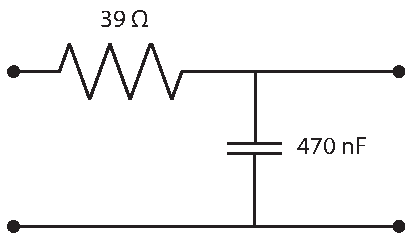
\includegraphics[angle=0,scale=0.5]{bilder/LPfilter.pdf}
  \caption{Lågpassfilter}
  \label{fig:lagpassfilter}
\end{figure}


\subsubsection{Upptäckning av korsningar och 90\degree svängar}
\label{sec:upptackkorsning}
Enligt specifikationen av den bana som roboten ska kunna följa, framgår det 
att det före alla korsningar ska finnas tejpmarkeringar som visar i vilken 
riktning roboten ska svänga, se \ref{sec:riktmark}. Roboten kommer att 
upptäcka korsningar om två av riktningarna höger, vänster och framåt visar 
mer än 80 cm.

Roboten kommer att upptäcka 90\degree svängar om det är längre än 80 cm åt 
höger eller vänster(inte båda), samt mindre än 35cm framåt.

Upptäcker roboten en korsning kommer det kommando som beskrivits av tidigare 
tejpmarkeringar att skickas till styrenheten. Datat som skickas är skrivet 
för att uppfattas som ett så kallat specialkommando, det vill säga 
styrenheten har en procedur som utförs utan att ta hänsyn till den reglerdata 
som skickas från sensorenheten. Märk att detta specialkommando innehåller en 
framkörning till mitten av korsningen, till skillnad från 90\degree svängar 
som utförs omedelbart.

Upptäcker korsningen en 90\degree sväng kommer ett annat specialkommando att 
utföras, där roboten svänger 90\degree åt det håll som avståndssensorerna 
visar har det längre avståndet.


\subsubsection{Display}
Robotens display-enhet är av typ \emph{LCD JM162A}. Displayen används för att visa avståndssensorernas värden. Eftersom sensorerna bara kan ge korrekta värden i intervallet 20-120 cm så kommer även displayen arbeta i detta intervall. Displayen arbetar i åtta databitarsläge och visar två rader med tecken. 

%Pinnar
Förutom de åtta databitarna som överförs för varje tecken till displayen så går ytterligare två signaler mellan sensorenhetens mikroprocessor och displayenheten: \emph{Enable} och \emph{Register select}. Enable-signalen signalerar till displayen att något ska skrivas ut, och Register select väljer mellan input-lägena 'data' och 'function'. Då det aldrig är någon data som läses från displayen så är pinnen \emph{R/W} konstant låg. 

%Kod
Sensorenheten har två funktioner som kan kallas för att skriva ut ett tecken på displayen. I funktionen \emph{char\_to\_display} anges parmetrarna vilket tecken (givet i ASCII-kod) som ska skrivas ut, samt vilken position på displayen som ska skrivas till. Denna funktion används för bokstäver. För att skriva ut sensorvärden används funktionen \emph{data\_to\_display}, vilken tar parametrarna för sensorvärdet i cm samt vilken sensor som skickat det. 

Sensorprocessorn har också en funktion för att konvertera cm-värdet till ASCII-kod, vilken används av \emph{data\_to\_display}.

\subsection{Mjukvara}

\subsubsection{AD}

\subsubsection{Linjesensor}


\subsubsection{Avståndsberäkning}


\subsubsection{Kommunikation}


\section{Styrenhet}

\subsection{Hårdvara}

\begin{figure}[H]
  \centering
 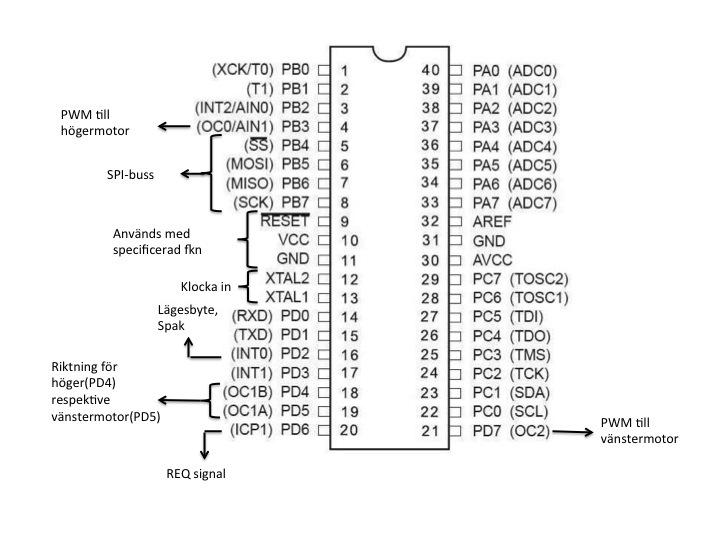
\includegraphics[angle=0,scale=0.5]{bilder/PIN_styr.jpg}
  \caption{Styrenhetens pin-anslutningar}
  \label{fig:PINstyr}
\end{figure}


\subsection{Mjukvara}

\subsubsection{Autonomt läge}

\subsection{Reglering}
Två olika regleralgoritmer används i roboten, en när roboten följer linjer och
en när roboten kör i labyrinter.
\subsubsection{Linjereglering}
TODO: Linjereglering
\subsubsection{Labyrintreglering}
Labyrintregleringen består av 3 olika delar med olika vikter,
en del som ser till att roboten går rakt (P-del), en del som ser till att
roboten håller sig i mitten av labyrinten (M-del) och en del som motverkar
svängningar (D-del).


P-delen använder sig av sidosensorerna för att hålla roboten parallell med
labyrintväggen. En vägg följs i taget, och kommer roboten för nära en vägg så
följs istället den andra väggen. Detta är den huvudsakliga regleringen och har
hög vikt.


M-delen använder sig av frontsensorerna för att hålla sig i mitten av
labyrinten, den försöker att hålla skillnaden mellan höger- och vänstersensorn
till 0. Om det bara finns en vägg att reglera på avaktiveras denna del. Då det
inte är helt avgörande om roboten är i mitten eller lite åt sidan i labyrinten
har denna del låg vikt.


D-delen ser till att roboten rör sig lugnt och inte börjar att oscillera i
labyrinten. Detta gör den genom att kika på skillnaden på sidosensorerna och är
den skillnaden stor så motverkar den P-delen. Eftersom D-delen reglerar på
relativt små skillnader har den hög vikt.

\label{reglering}

 % #6 -Detaljerat om varje modul
	%% Innehåller komm.tex, pcmjuk.tex, sensor.tex, styr.tex
% !TEX encoding = UTF-8 Unicode

%% --------------------------------------------------------------------------------------------------------------------------------------------
% SLUTSATS - Möjliga förbättringar samt utvecklingsmöjligheter
%
% --matja307, 2012-05-06
%% --------------------------------------------------------------------------------------------------------------------------------------------

\section{Slutsats}

Todo: Något om möjliga förbättringar och vidareutveckling.

 % #7 -Förbättringspotential etc.
\section{Referenser}
 % #8 -Referenser
%% --------------------------------------------------------------------------------------------------------------------------------------------
% APPENDIX - Blindtarm
%
% --matja307, 2012-05-06
%% --------------------------------------------------------------------------------------------------------------------------------------------

\section*{Appendix}
\appendix

\addcontentsline{toc}{section}{Appendix}

\lstset{inputencoding=utf8,
        language=c,
        linewidth=\textwidth,
        basicstyle=\scriptsize,
        numbers=left,
        stepnumber=1,
        tabsize=8,
        showtabs=false
}
\lstset{literate={å}{{\aa}}1
                {ä}{{\"a}}1
                {ö}{{\"o}}1
                {Å}{{\AA}}1
                {Ä}{{\"A}}1
                {Ö}{{\"O}}1
}


\section{Omvandlingsdiagram}
\label{appendix:cmomvandling}


\begin{figure}[H]
  \centering
 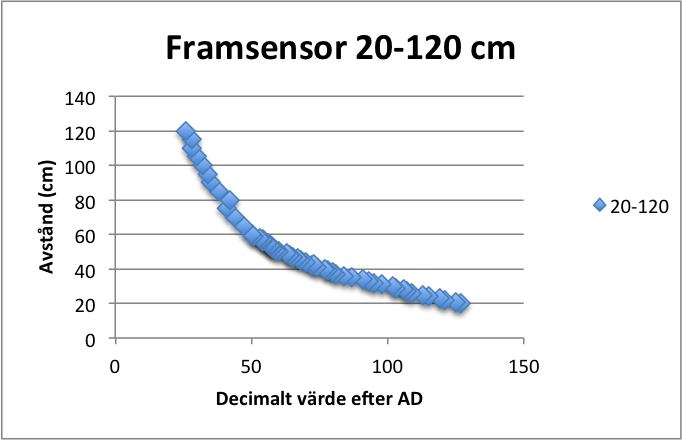
\includegraphics[angle=0,scale=1]{bilder/F_20_120.png}
  \caption{Framsensorn omvandling 20-120}
\end{figure}

\begin{figure}[H]
  \centering
 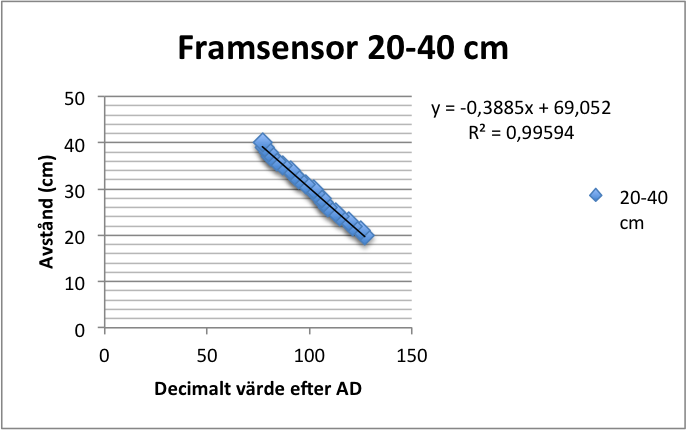
\includegraphics[angle=0,scale=1]{bilder/F_20_40.png}
  \caption{Framsensorn omvandling 20-40}
\end{figure}

\begin{figure}[H]
  \centering
 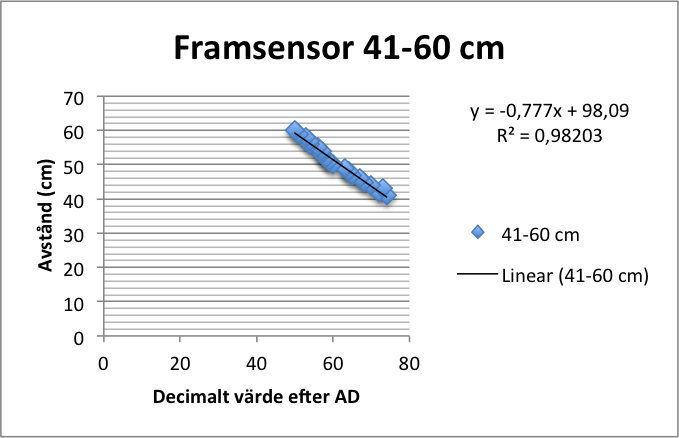
\includegraphics[angle=0,scale=1]{bilder/F_41_60.png}
  \caption{Framsensorns omvandling 41-60}
\end{figure}

\begin{figure}[H]
  \centering
 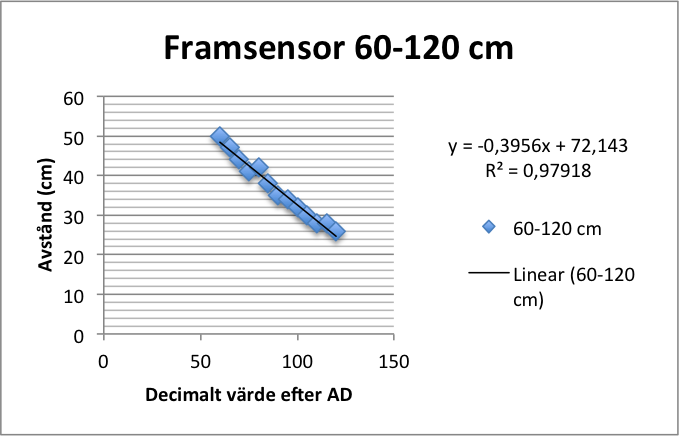
\includegraphics[angle=0,scale=1]{bilder/F_60_120.png}
  \caption{Framsensorn omvandling 60-120}
\end{figure}

\begin{figure}[H]
  \centering
 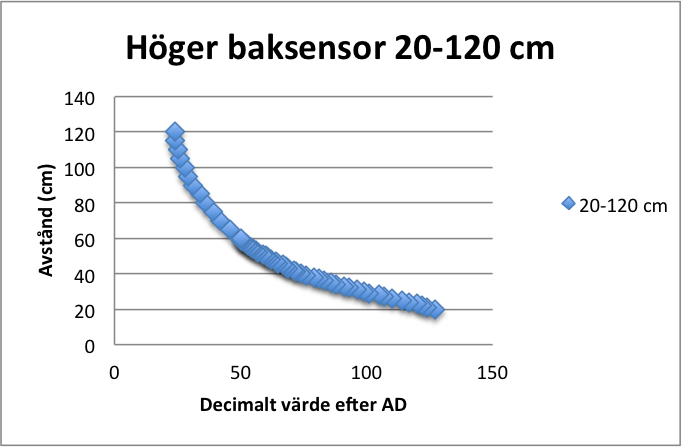
\includegraphics[angle=0,scale=1]{bilder/HB_20_120.png}
  \caption{Höger baksensor 20-120}
\end{figure}

\begin{figure}[H]
  \centering
 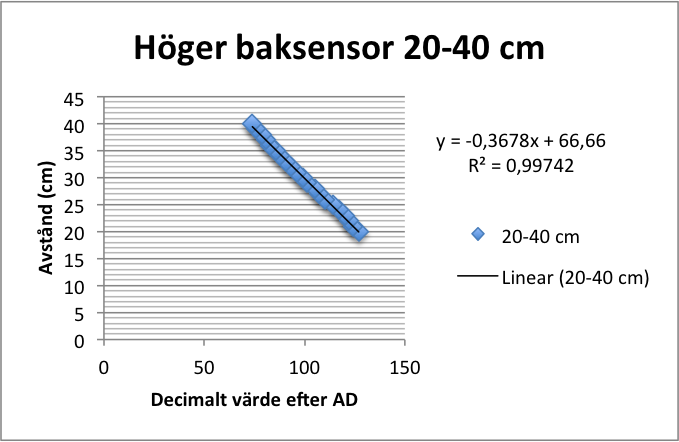
\includegraphics[angle=0,scale=1]{bilder/HB_20_40.png}
  \caption{Höger baksensor 20-40}
\end{figure}

\begin{figure}[H]
  \centering
 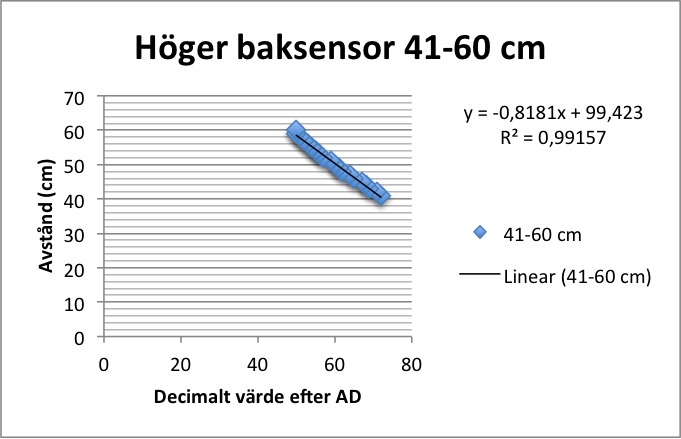
\includegraphics[angle=0,scale=1]{bilder/HB_41_60.png}
  \caption{Höger baksensor 41-60}
\end{figure}

\begin{figure}[H]
  \centering
 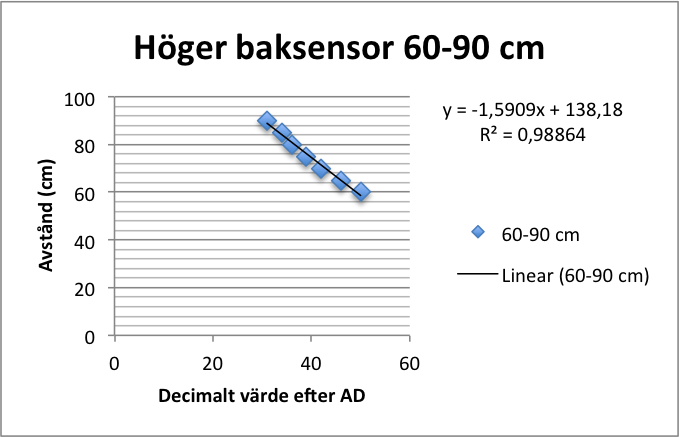
\includegraphics[angle=0,scale=1]{bilder/HB_60_90.png}
  \caption{Höger baksensor 60-90}
\end{figure}

\begin{figure}[H]
  \centering
 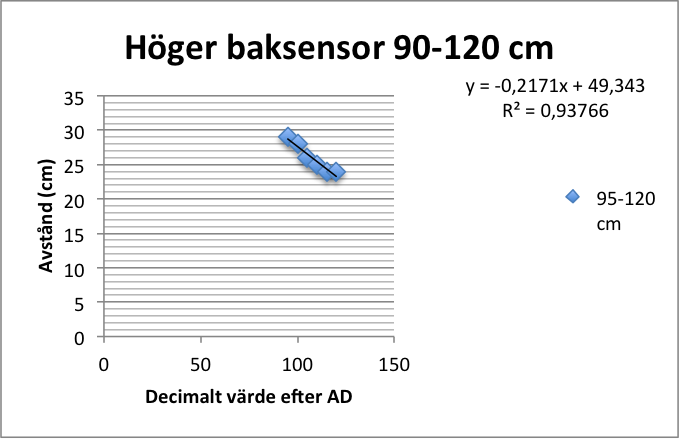
\includegraphics[angle=0,scale=1]{bilder/HB_90_120.png}
  \caption{Höger baksensor 90-120}
\end{figure}

\begin{figure}[H]
  \centering
 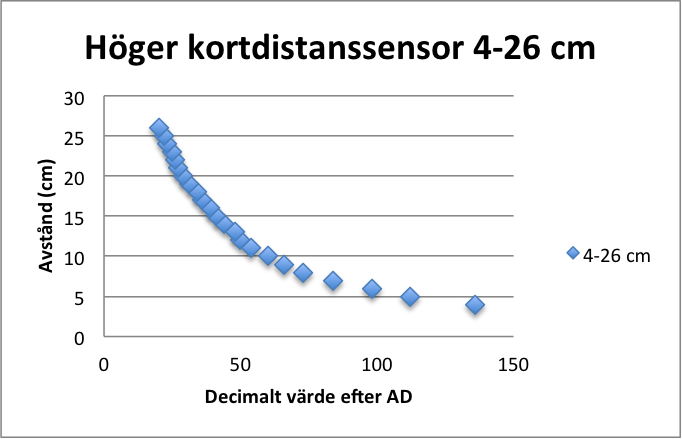
\includegraphics[angle=0,scale=1]{bilder/H_K_4_26.png}
  \caption{Höger kortdistanssensor 4-26}
\end{figure}

\begin{figure}[H]
  \centering
 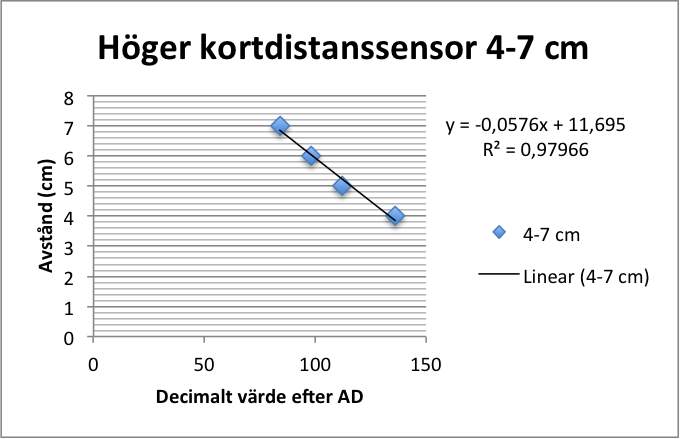
\includegraphics[angle=0,scale=1]{bilder/H_K_4_7png.png}
  \caption{Höger kortdistanssensor 4-7}
\end{figure}

\begin{figure}[H]
  \centering
 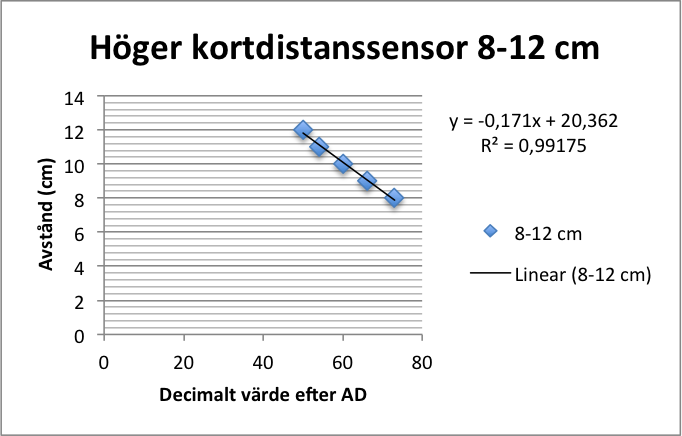
\includegraphics[angle=0,scale=1]{bilder/H_K_8_12.png}
  \caption{Höger kortdistanssensor 8-12}
\end{figure}

\begin{figure}[H]
  \centering
 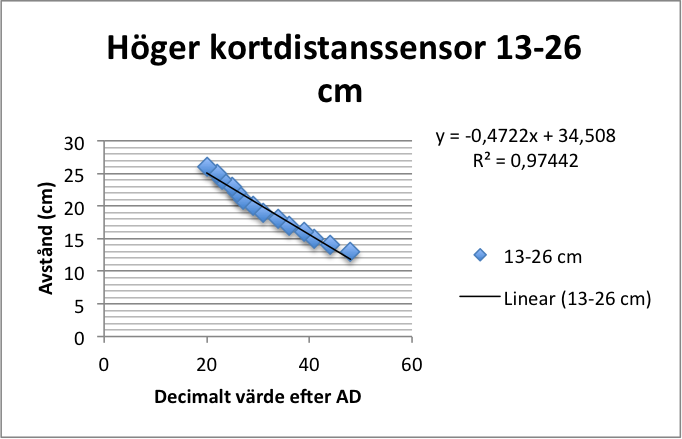
\includegraphics[angle=0,scale=1]{bilder/H_K_13_26.png}
  \caption{Höger kortdistanssensor 13-26}
\end{figure}

\begin{figure}[H]
  \centering
 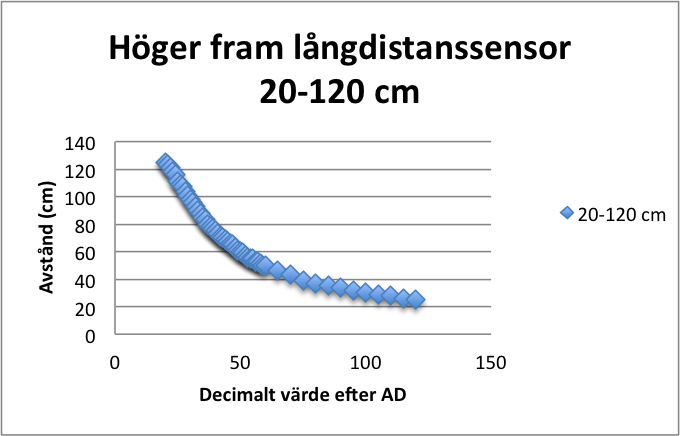
\includegraphics[angle=0,scale=1]{bilder/HF_20_120.png}
  \caption{Höger framsensor 20-120}
\end{figure}

\begin{figure}[H]
  \centering
 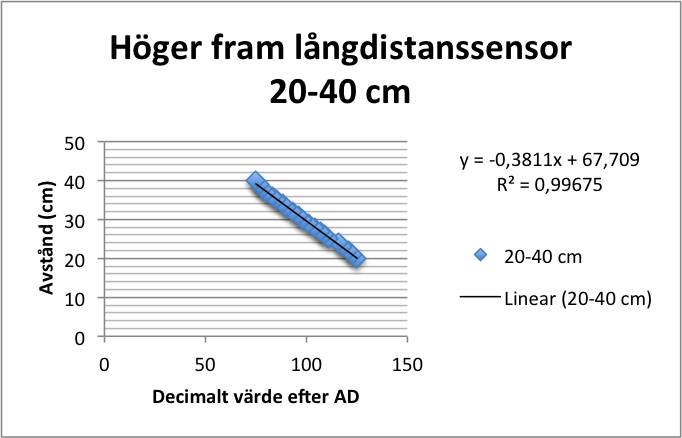
\includegraphics[angle=0,scale=1]{bilder/HF_20_40.png}
  \caption{Höger framsensor 20-40}
\end{figure}

\begin{figure}[H]
  \centering
 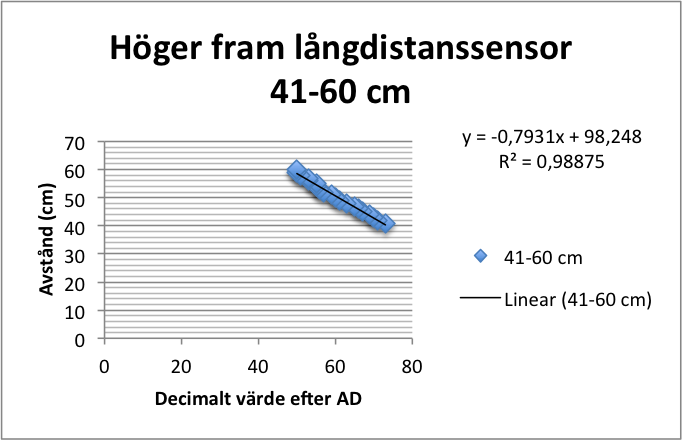
\includegraphics[angle=0,scale=1]{bilder/HF_41_60.png}
  \caption{Höger framsensor 41-60}
\end{figure}

\begin{figure}[H]
  \centering
 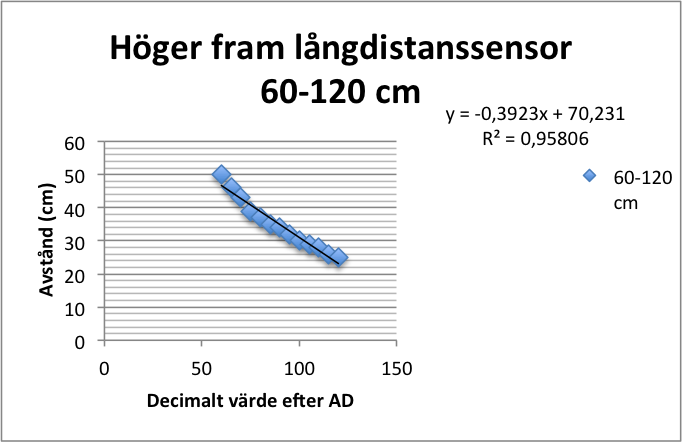
\includegraphics[angle=0,scale=1]{bilder/HF_60_120.png}
  \caption{Höger framsensor 60-120}
\end{figure}

\begin{figure}[H]
  \centering
 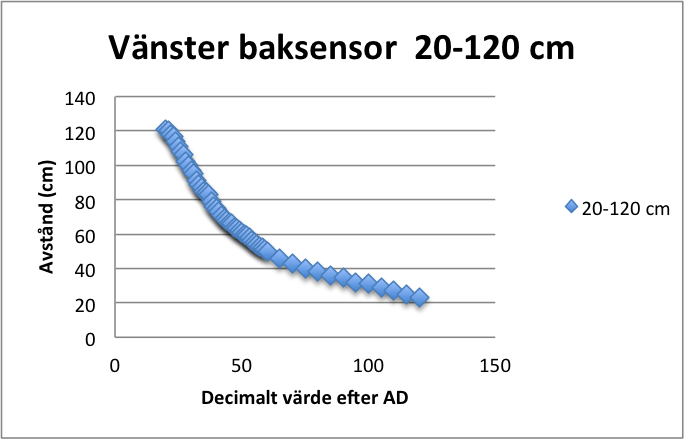
\includegraphics[angle=0,scale=1]{bilder/VB_20_120.png}
  \caption{Vänster baksensor 20-120}
\end{figure}

\begin{figure}[H]
  \centering
 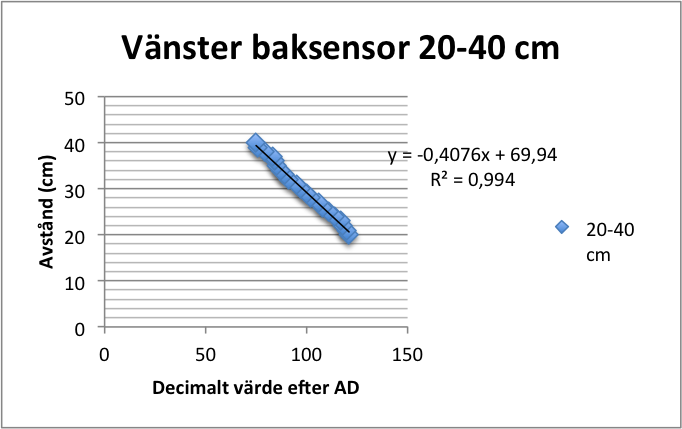
\includegraphics[angle=0,scale=1]{bilder/VB_20_40.png}
  \caption{Vänster baksensor 20-40}
\end{figure}


\begin{figure}[H]
  \centering
 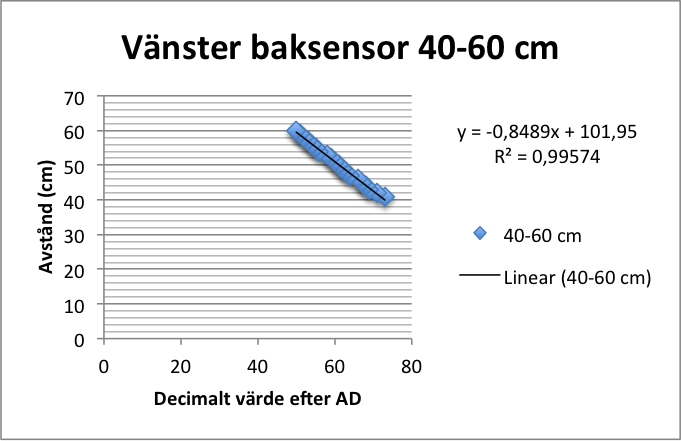
\includegraphics[angle=0,scale=1]{bilder/VB_40_60.png}
  \caption{Vänster baksensor 40-60}
\end{figure}

\begin{figure}[H]
  \centering
 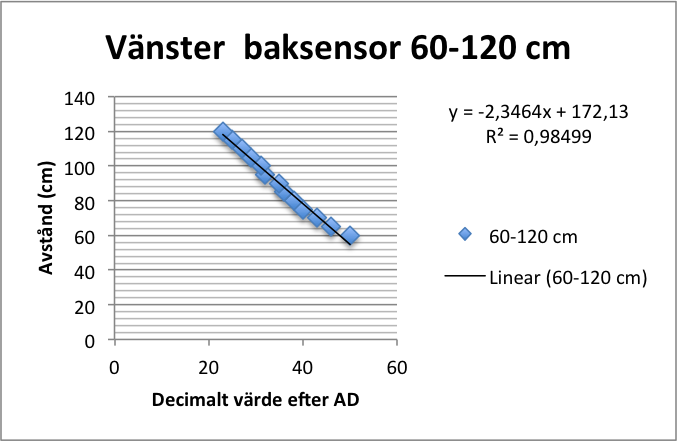
\includegraphics[angle=0,scale=1]{bilder/VB_60_120.png}
  \caption{Vänster baksensor 60-120}
\end{figure}

\begin{figure}[H]
  \centering
 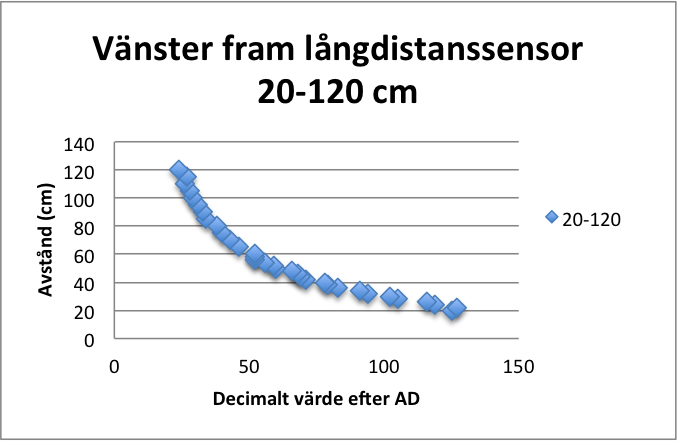
\includegraphics[angle=0,scale=1]{bilder/VF_20_120.png}
  \caption{Vänster framsensor 20-120}
\end{figure}

\begin{figure}[H]
  \centering
 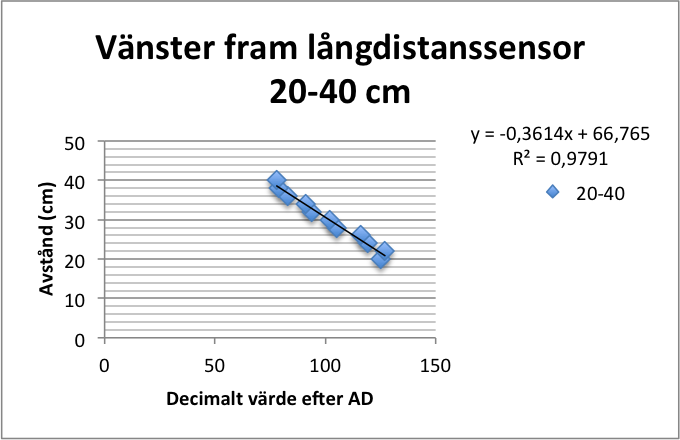
\includegraphics[angle=0,scale=1]{bilder/VF_20_40.png}
  \caption{Vänster framsensor 20-40}
\end{figure}

\begin{figure}[H]
  \centering
 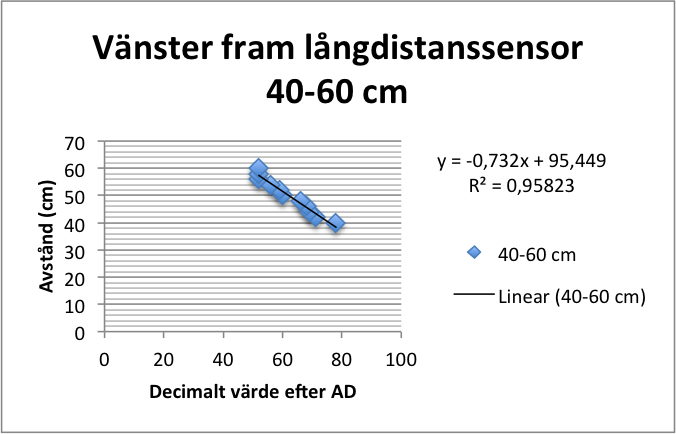
\includegraphics[angle=0,scale=1]{bilder/VF_40_60.png}
  \caption{Vänster framsensor 40-60}
\end{figure}

\begin{figure}[H]
  \centering
 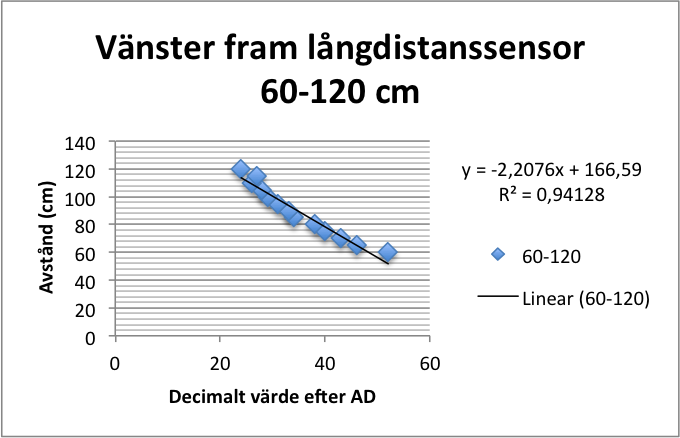
\includegraphics[angle=0,scale=1]{bilder/VF_60_120.png}
  \caption{Vänster framsensor 60-120}
\end{figure}






\subsection*{A \hspace*{1em} Kod}
\addcontentsline{toc}{subsection}{A \hspace*{1em} Kod}


%%%%%%%%%%%%%%%%%%%%%%%%%%%%%%%%%%%%%%%%%%%%%%%%%%%%%%%%%%%%%%%%%%%%%%%%%%%%%%%
% PC
% Kod till användargränssnittet
%%%%%%%%%%%%%%%%%%%%%%%%%%%%%%%%%%%%%%%%%%%%%%%%%%%%%%%%%%%%%%%%%%%%%%%%%%%%%%%
\subsubsection*{A.1 \hspace*{1em} PC}
\addcontentsline{toc}{subsubsection}{A.1 \hspace*{1em} PC}
\lstinputlisting[caption=input\_control,label=lst:input]{../../Kod/pc/input_control.c}
\lstinputlisting[caption=keypress.h,label=lst:keypress_h]{../../Kod/pc/keypress.h}
\lstinputlisting[caption=keypress.c,label=lst:keypress_c]{../../Kod/pc/keypress.c}
\lstinputlisting[caption=header.h,label=lst:header_h]{../../Kod/pc/header.h}
\lstinputlisting[caption=header.c,label=lst:header_c]{../../Kod/pc/header.c}
\lstinputlisting[caption=send\_receive.c,label=lst:sendrec_c]{../../Kod/pc/send_receive.c}
\lstinputlisting[caption=blue\_pc.h,label=lst:blue_h]{../../Kod/pc/blue_pc.h}
\lstinputlisting[caption=blue\_pc.c,label=lst:blue_c]{../../Kod/pc/blue_pc.c}
\lstinputlisting[caption=db.h,label=lst:db_h]{../../Kod/pc/db.h}
\lstinputlisting[caption=db.c,label=lst:db_c]{../../Kod/pc/db.c}
\lstinputlisting[caption=display.h,label=lst:display_h]{../../Kod/pc/display.h}
\lstinputlisting[caption=display.c,label=lst:display_c]{../../Kod/pc/display.c}

%%%%%%%%%%%%%%%%%%%%%%%%%%%%%%%%%%%%%%%%%%%%%%%%%%%%%%%%%%%%%%%%%%%%%%%%%%%%%%%
% Kommunikationsenhet
%%%%%%%%%%%%%%%%%%%%%%%%%%%%%%%%%%%%%%%%%%%%%%%%%%%%%%%%%%%%%%%%%%%%%%%%%%%%%%%
\subsubsection*{A.2 \hspace*{1em} Kommunikationsenhet}
\addcontentsline{toc}{subsubsection}{A.2 \hspace*{1em} Kommunikationsenhet}
\lstinputlisting[caption=komm\_main.c,label=lst:komm_main_c]{../../Kod/komm/komm_main.c}
\lstinputlisting[caption=komm\_init.c,label=lst:komm_init_c]{../../Kod/komm/komm_init.c}
\lstinputlisting[caption=bluetooth\_interrupt.c,%
label=lst:bluetooth_interrupt_c]{../../Kod/komm/bluetooth_interrupt.c}
\lstinputlisting[caption=komm\_SPI.c,label=lst:komm_SPI_c]{../../Kod/komm/komm_SPI.c}

%%%%%%%%%%%%%%%%%%%%%%%%%%%%%%%%%%%%%%%%%%%%%%%%%%%%%%%%%%%%%%%%%%%%%%%%%%%%%%%
% Styrenehet
%%%%%%%%%%%%%%%%%%%%%%%%%%%%%%%%%%%%%%%%%%%%%%%%%%%%%%%%%%%%%%%%%%%%%%%%%%%%%%%
\subsubsection*{A.3 \hspace*{1em} Styrenhet}
\addcontentsline{toc}{subsubsection}{A.3 \hspace*{1em} Styrenhet}
\lstinputlisting[caption=styr\_main.c,label=lst:styr_main_c]{../../Kod/styr/styr_main.c}
\lstinputlisting[caption=motor\_styrning.h,label=lst:motor_styrning_h]{../../Kod/styr/motor_styrning.h}
\lstinputlisting[caption=motor\_styrning.c,label=lst:motor_styrning_c]{../../Kod/styr/motor_styrning.c}
\lstinputlisting[caption=regulator.h,label=lst:regulator_h]{../../Kod/styr/regulator.h}
\lstinputlisting[caption=regulator.c,label=lst:regulator_c]{../../Kod/styr/regulator.c}
\lstinputlisting[caption=styr\_specialkommando.h,label=lst:styr_specialkommando_h]{../../Kod/styr/styr_specialkommando.h}
\lstinputlisting[caption=styr\_specialkommando.c,label=lst:styr_specialkommando_c]{../../Kod/styr/styr_specialkommando.c}
\lstinputlisting[caption=styr\_tolka\_data.h,label=lst:styr_tolka_data_h]{../../Kod/styr/styr_tolka_data.h}
\lstinputlisting[caption=styr\_tolka\_data.c,label=lst:styr_tolka_data_c]{../../Kod/styr/styr_tolka_data.c}
\lstinputlisting[caption=styr\_SPI.h,label=lst:styr_SPI_h]{../../Kod/styr/styr_SPI.h}
\lstinputlisting[caption=styr\_SPI.c,label=lst:styr_SPI_c]{../../Kod/styr/styr_SPI.c}

%%%%%%%%%%%%%%%%%%%%%%%%%%%%%%%%%%%%%%%%%%%%%%%%%%%%%%%%%%%%%%%%%%%%%%%%%%%%%%%
% Sensorenhet
%%%%%%%%%%%%%%%%%%%%%%%%%%%%%%%%%%%%%%%%%%%%%%%%%%%%%%%%%%%%%%%%%%%%%%%%%%%%%%%
\subsubsection*{A.4 \hspace*{1em} Sensorenhet}
\addcontentsline{toc}{subsubsection}{A.4 \hspace*{1em} Sensorenhet}
\lstinputlisting[caption=sensor.c,label=lst:sensor_c]{../../Kod/sensor/sensor.c}
\lstinputlisting[caption=sensor\_init.h,label=lst:sensor_init_h]{../../Kod/sensor/sensor_init.h}
\lstinputlisting[caption=sensor\_init.c,label=lst:sensor_init_c]{../../Kod/sensor/sensor_init.c}
\lstinputlisting[caption=sensor\_ad.h,label=lst:sensor_ad_h]{../../Kod/sensor/sensor_ad.h}
\lstinputlisting[caption=sensor\_ad.c,label=lst:sensor_ad_c]{../../Kod/sensor/sensor_ad.c}
\lstinputlisting[caption=sensorvarde\_omvandling.h,label=lst:sensorvarde_omvandling_h]{../../Kod/sensor/sensorvarde_omvandling.h}
\lstinputlisting[caption=sensorvarde\_omvandling.c,label=lst:sensorvarde_omvandling_c]{../../Kod/sensor/sensorvarde_omvandling.c}
\lstinputlisting[caption=displayenhet.h,label=lst:displayenhet_h]{../../Kod/sensor/displayenhet.h}
\lstinputlisting[caption=displayenhet.c,label=lst:displayenhet_c]{../../Kod/sensor/displayenhet.c}
\lstinputlisting[caption=linjeskillnad.h,label=lst:linjeskillnad_h]{../../Kod/sensor/linjeskillnad.h}
\lstinputlisting[caption=linjeskillnad.c,label=lst:linjeskillnad_c]{../../Kod/sensor/linjeskillnad.c}
\lstinputlisting[caption=upptack\_tejp.h,label=lst:upptack_tejp_h]{../../Kod/sensor/upptack_tejp.h}
\lstinputlisting[caption=upptack\_tejp.c,label=lst:upptack_tejp_c]{../../Kod/sensor/upptack_tejp.c}
\lstinputlisting[caption=special.h,label=lst:special_h]{../../Kod/sensor/special.h}
\lstinputlisting[caption=special.c,label=lst:special_c]{../../Kod/sensor/special.c}
\lstinputlisting[caption=sensor\_spi.h,label=lst:sensor_spi_h]{../../Kod/sensor/sensor_spi.h}
\lstinputlisting[caption=sensor\_spi.c,label=lst:sensor_spi_c]{../../Kod/sensor/sensor_spi.c}

\subsection*{B \hspace*{1em} Kopplingsschema}
\addcontentsline{toc}{subsection}{B \hspace*{1em} Kopplingsschema}
\begin{figure}[H]
 \centering
 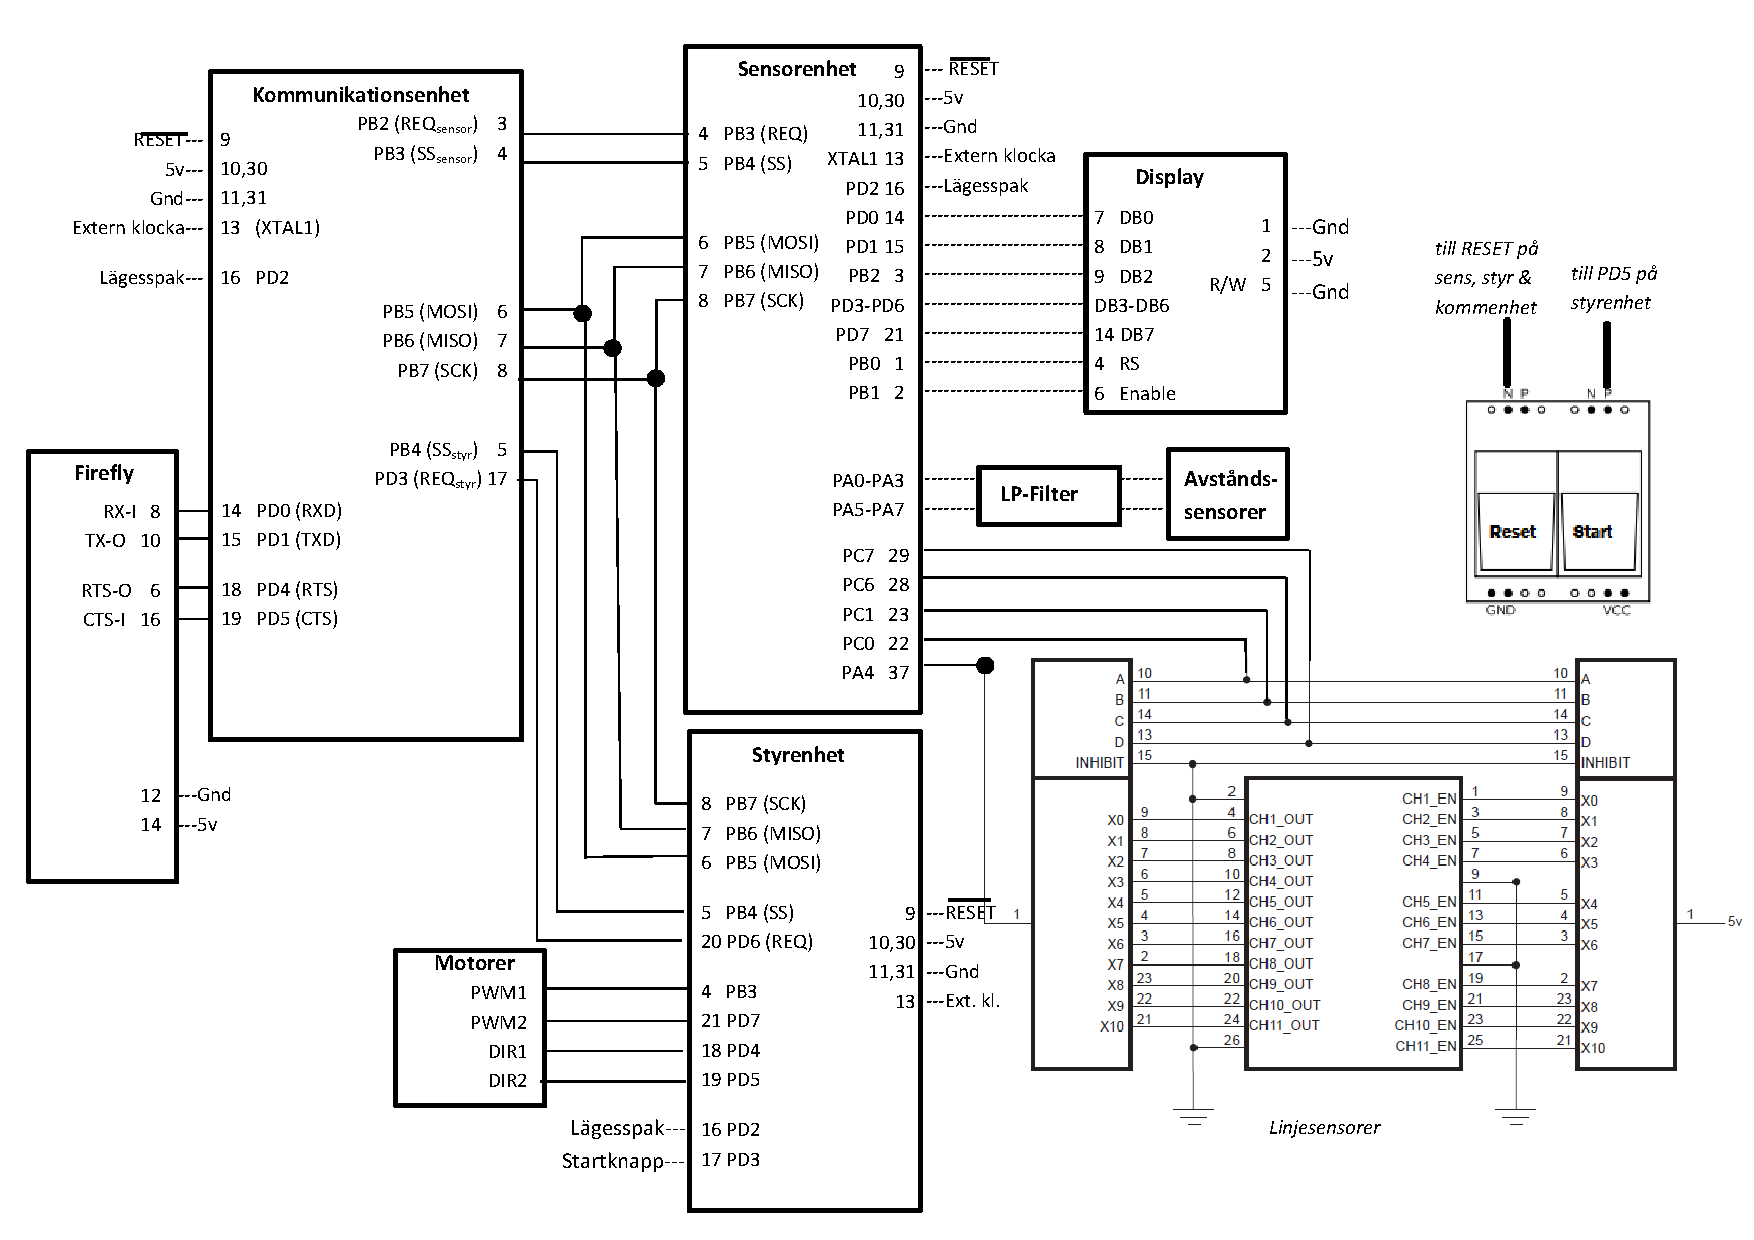
\includegraphics[angle=270,scale=0.75]{bilder/kopplingsschema.pdf}
  \caption{Kopplingsschema för systemet}
  %\label{fig:system}
\end{figure}
 % -Appendix

\newpage
\end{document} 

%%% Local Variables: 
%%% mode: latex
%%% TeX-master: t
%%% End: 
